% ID: SEL-D0013-BA-E02
% ESTADO: validada. S014; tres pasadas del mismo autor, sin segundo revisor.
\textbf{a) Intersección de semiplanos.}\par\nopagebreak[4]
Despejamos $y$:
\[
y\leq\frac{13-x}{2},\quad y\geq x-4,\quad
y\leq\frac{x+7}{2},\quad y\geq5-x.
\]
No se añaden restricciones de no negatividad. Las intersecciones factibles, en orden alrededor del recinto, son
\[
\boxed{(1,4),\quad(9/2,1/2),\quad(7,3),\quad(3,5).}
\]
Se obtienen de las parejas de fronteras tercera/cuarta, segunda/cuarta, primera/segunda y primera/tercera, respectivamente. Las otras intersecciones se descartan por incumplir alguna desigualdad. El recinto es cerrado y acotado.
\begin{center}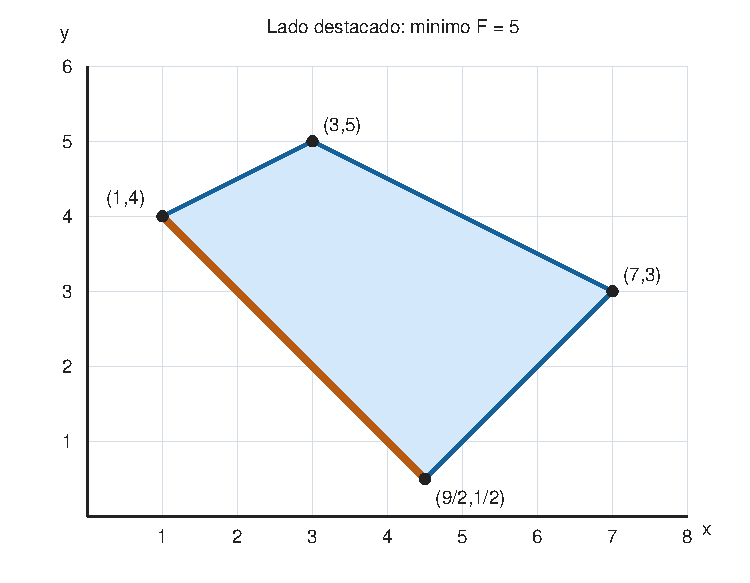
\includegraphics[width=0.58\linewidth]{recursos/figuras/s014-region.pdf}\end{center}

\textbf{b) Extremos y todos los puntos que los alcanzan.}\par\nopagebreak[4]
Evaluamos la función lineal en los vértices:
\[
\begin{array}{c|rrrr}
(x,y)&(1,4)&(9/2,1/2)&(7,3)&(3,5)\\\hline
F=x+y&5&5&10&8
\end{array}
\]
El \textbf{máximo} es \boxed{10\text{, únicamente en }(7,3)}. Se comprueba globalmente combinando la primera restricción con la segunda:
\[
x+y=\frac23(x+2y)+\frac13(x-y)\leq\frac{26+4}{3}=10.
\]
La igualdad fuerza ambas fronteras y determina ese vértice. El \textbf{mínimo} es \boxed{5}, alcanzado en \textbf{todo el segmento} de $(1,4)$ a $(9/2,1/2)$:
\[
\boxed{(x,y)=\left(1+\frac72t,\ 4-\frac72t\right),\quad0\leq t\leq1.}
\]
La cuarta restricción garantiza $F\geq5$, y la igualdad $x+y=5$ dentro del recinto es exactamente ese lado. No basta con dar sólo los dos vértices extremos del segmento.
